\chapter{Lecture 10: New Revolutions in Particle Physics}

These notes follow Leonard Susskind's tenth lecture in the supplementary Particle Physics 2 sequence, with curation by LazyingArt LLC, and they keep the argument in the order in which the lecture actually unfolds. Susskind begins by looking ahead to the larger puzzles of the Standard Model, to unification, supersymmetry, the LHC, and above all to the gauge-hierarchy problem. That opening is not ornamental. It tells us why the Higgs is being brought back into focus. The Higgs is not merely one more particle to be discovered; it is the device by which the theory organizes masses and couplings, and therefore the place where mathematical consistency and the larger ultraviolet puzzles come into direct contact.

\section{From Higgs Motivation Back to the Dirac Lagrangian}

If one of the original aims of the LHC was to discover the Higgs boson, then discovering the Higgs would mean more than finding a resonance. It would mean uncovering a whole pattern of masses and interactions associated with that field. To reach that point, Susskind backs up from Higgs phenomenology to the Dirac equation and, more precisely, to the Dirac Lagrangian. That move is typical of the lecture: before we can talk seriously about fermion masses, we must first look carefully at the operator that a mass term actually is.

He begins with the older \(\alpha,\beta\) notation on the blackboard.

\begin{figure}[h]
\centering

\includegraphics[width=0.82\textwidth]{lecture_10_figure_02.png}
\caption{Dirac Lagrangian in \(\alpha,\beta\) notation.}
\end{figure}

The board expression is partially cropped and loose about signs and \(i\)-factors, so we keep only the structure that is secure from the transcript. In the lecture's notation one starts schematically from
\begin{align}
\left(\partial_t+\alpha_i\partial_i-\beta m\right)\psi &= 0, \\
\mathcal{L}_D^{(\alpha,\beta)}
=
\psi^\dagger\left(\partial_t+\alpha_i\partial_i-\beta m\right)\psi .
\end{align}
The point here is not a fetish for an old notation. It is that the Lagrangian is being constructed directly from the equation of motion: multiply the Dirac equation by \(\psi^\dagger\), and the expression that varies back to the equation falls right out.

Susskind immediately interprets the terms. The derivative terms are kinetic terms. They absorb a particle at one point and move it to a neighboring point of spacetime; at the same time they act on spin. The mass term does no such moving. It absorbs and re-emits at the same point. At first sight that seems ordinary enough. But the lecture is heading toward the claim that, in a chiral weak theory, this innocent-looking term is not innocent at all.

He then cleans up the notation and translates to the covariant language. Define
\begin{equation}
\bar{\psi}=\psi^\dagger\beta=\psi^\dagger\gamma^0,
\qquad
\gamma^0\equiv \beta,
\qquad
\gamma^i\equiv \beta\alpha_i.
\end{equation}
With these conventions the Lagrangian becomes
\begin{equation}
\mathcal{L}_D
=
\bar{\psi}\left(\gamma^0\partial_t+\gamma^i\partial_i+m\right)\psi .
\end{equation}
The blackboard does not reliably fix the final sign convention or the explicit \(i\), so we standardize once and for all to the canonical modern form
\begin{equation}
\mathcal{L}_D
=
\bar{\psi}\left(i\gamma^\mu\partial_\mu-m\right)\psi .
\end{equation}

\begin{figure}[h]
\centering

\includegraphics[width=0.82\textwidth]{lecture_10_figure_03.png}
\caption{Covariant gamma-matrix form of the Dirac Lagrangian.}
\end{figure}

This rewrite is not cosmetic. It sets up the next move. In this language \(\bar{\psi}\psi\) is a scalar, while \(\bar{\psi}\gamma^\mu\psi\) is a four-vector. We can now inspect the terms and ask, in a cleaner language, what the mass term actually does.

\section{Chirality and the Meaning of a Dirac Mass}

The lecture now introduces the fifth Dirac matrix, \(\gamma_5\). Susskind briefly says ``helicity'' and then corrects himself to ``chirality,'' which is the concept that matters here. The operator satisfies
\begin{equation}
\gamma_5^2=1,
\end{equation}
and therefore has eigenvalues \(\pm1\). We may correspondingly split the spinor into its left- and right-chiral pieces:
\begin{equation}
\psi=\psi_L+\psi_R.
\end{equation}

The crucial fact, emphasized by Susskind, is that the kinetic part of the Dirac Lagrangian does not mix these two sectors, whereas the scalar mass term does. That is the mathematical hinge of the lecture.

\begin{figure}[h]
\centering

\includegraphics[width=0.80\textwidth]{lecture_10_figure_04.png}
\caption{Left-right decomposition of the Dirac mass term.}
\end{figure}

The key decomposition is
\begin{equation}
\bar{\psi}\psi
=
\psi_L^\dagger\psi_R+\psi_R^\dagger\psi_L .
\end{equation}
Thus the Dirac mass term is
\begin{equation}
-m\bar{\psi}\psi
=
-m\left(\psi_L^\dagger\psi_R+\psi_R^\dagger\psi_L\right).
\end{equation}
So a Dirac mass is not merely a parameter that one appends to the equation. It is an operator that flips left-handed fermions into right-handed ones and right-handed fermions back into left-handed ones. The kinetic terms do not do that. The mass term does.

This is where the lecture becomes mathematically sharp. A massless fermion can carry definite chirality. A massive fermion cannot remain in one chiral sector, because the mass term itself is a left-right mixing term. Once that point has been made, the collision with weak interactions is unavoidable.

\section{Weak Interactions and the Forbidden Mass Term}

Susskind now recalls that weak interactions are chiral. He first speaks of the \(Z\) and then corrects himself: for the present argument the relevant focus is the \(W\)-boson coupling. The \(W\) couples only to the left-handed degrees of freedom. So with respect to the weak \(SU(2)\) symmetry under discussion, the left-handed fermion is charged and the right-handed fermion is uncharged.

But the Dirac mass term takes
\[
\psi_L \longleftrightarrow \psi_R.
\]
In other words, it turns something weakly charged into something uncharged, and vice versa. That is not an allowed term in the weak gauge theory. It would violate the transformation law that the Lagrangian must respect. So the familiar bare mass term, perfectly natural in an abstract Dirac theory, becomes forbidden once the weak interaction is remembered to be chiral.

\subsection{Question \& Answer}

\paragraph{Question.} How can fermions be massive if the weak interaction couples only to left-handed fields?

\paragraph{Answer.} By themselves, they cannot be given a bare Dirac mass without violating the weak gauge symmetry. The left-right mixing must instead be promoted to a new interaction in which an additional field carries the weak charge mismatch. That additional field is the Higgs field.

This is one of the lecture's most characteristic beats. A standard term is not simply declared illegal and replaced by a textbook formula. Rather, the symmetry obstruction is made explicit first. Only then is the Higgs introduced as the repair.

\section{Higgs Insertion, Yukawa Couplings, and Observable Consequences}

The Higgs field now enters in exactly the way the previous section has prepared us to expect. It carries the weak charge that the mass term could not otherwise balance. Susskind notes that the Higgs is itself a weak doublet, but he deliberately does not stop to unpack its full component structure. The lecture stays schematic, because the structural point is already visible without the full Standard Model index machinery.

On the board the Higgs-assisted left-right coupling appears together with the first sketch of the Higgs potential. That juxtaposition is faithful to the lecture: the Higgs is introduced first as the repair of the fermion-mass obstruction and immediately thereafter as a dynamical field whose own potential must be understood.

\begin{figure}[h]
\centering

\includegraphics[width=0.78\textwidth]{lecture_10_figure_05.png}
\caption{The board now carries both the Higgs-assisted chiral coupling and the first sketch of the symmetry-breaking potential.}
\end{figure}

The cleaned schematic Yukawa interaction is
\begin{equation}
\mathcal{L}_Y
=
G_Y\left(\psi_L^\dagger \phi\,\psi_R+\psi_R^\dagger \phi^\dagger \psi_L\right),
\end{equation}
where \(G_Y\) is a dimensionless Yukawa coupling. Different fermions have different Yukawa couplings; the lecture treats them as inputs to the Lagrangian.

At this stage Susskind still says, in effect, that this would be the end of the story except for spontaneous symmetry breaking. The Higgs field does not remain at \(\phi=0\). Instead we write
\begin{equation}
\phi = F + H,
\end{equation}
where \(F\) is the nonfluctuating shifted value of the field and \(H\) is the Higgs fluctuation. Substituting into the Yukawa term gives
\begin{align}
\mathcal{L}_Y
&=
G_Y\left(\psi_L^\dagger(F+H)\psi_R+\psi_R^\dagger(F+H)^\dagger\psi_L\right) \\
&=
G_YF\left(\psi_L^\dagger\psi_R+\psi_R^\dagger\psi_L\right)
+
G_YH\left(\psi_L^\dagger\psi_R+\psi_R^\dagger\psi_L\right).
\end{align}
The first term is now a genuine fermion mass term, so we read off
\begin{equation}
m_f = G_YF.
\end{equation}
The second term is the Higgs-fermion interaction.

That is the real repair mechanism. The forbidden bare Dirac mass is replaced by a gauge-invariant Yukawa coupling, and after symmetry breaking the vacuum value \(F\) converts part of that interaction into an effective mass.

Susskind immediately emphasizes the predictive content. The same \(F\) that enters the \(W\) and \(Z\) masses enters the fermion masses as well. Since the weak-boson masses are known, one infers that
\begin{equation}
F \sim 200\,\mathrm{GeV},
\end{equation}
up to the rough lecture-level normalization. Then the observed fermion masses tell us the Yukawa couplings: a tiny electron mass means a tiny Yukawa coupling, while the large top mass means a large one.

And the same couplings govern Higgs decays. At the level of a schematic amplitude,
\begin{equation}
\mathcal{A}(H\to f\bar f)\propto G_Y,
\qquad
\Gamma(H\to f\bar f)\propto G_Y^2
\end{equation}
up to the usual kinematic factors and phase-space integrals. So the heavier the fermion, the larger the corresponding Yukawa coupling, and therefore the stronger the Higgs coupling to that channel. This is why discovering the Higgs would mean discovering more than one particle: it would reveal a network of couplings whose strengths are already encoded in the observed masses.

\section{The Mexican-Hat Potential and the Scale \(F\)}

Once masses have been generated, the lecture turns immediately to the dynamics of the Higgs field itself. Why does \(\phi\) acquire the shift \(F\)? Susskind's answer is: because the Higgs potential has the now-familiar Mexican-hat form.

We keep the board evidence visible here, because the same frame that carries the Yukawa coupling also carries the first unmistakable one-dimensional cross-section of the double-well potential.

\begin{figure}[h]
\centering

\includegraphics[width=0.78\textwidth]{lecture_10_figure_05.png}
\caption{Board evidence for the one-dimensional cross-section of the symmetry-breaking potential.}
\end{figure}

Near the origin the potential must be an upside-down parabola. The lecture writes it in the form
\begin{equation}
V(\phi)
=
-\frac{\mu^2}{2}\phi^2+\frac{\lambda}{4}\phi^4.
\end{equation}
This form is motivated step by step. The negative quadratic term makes the origin unstable. If that were the whole story, the field would simply run away to infinity and there would be no ground state at all. We therefore need a positive term that takes over at large \(|\phi|\) and turns the potential back upward. The simplest symmetric choice is the quartic term. Odd powers would spoil the symmetry between \(+\phi\) and \(-\phi\), and higher even powers are not needed for the first renormalizable stabilization.

\begin{figure}[h]
\centering
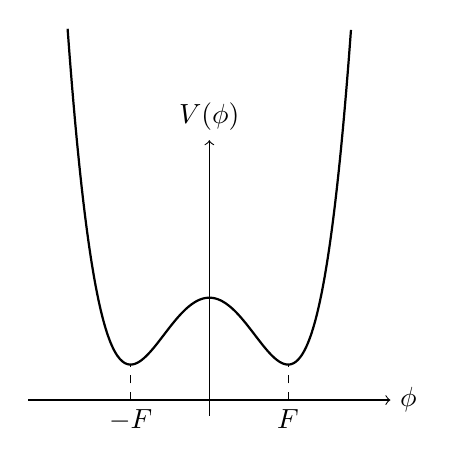
\begin{tikzpicture}[scale=1.0]
\draw[->] (-2.3,0) -- (2.3,0) node[right] {\(\phi\)};
\draw[->] (0,-0.2) -- (0,3.3) node[above] {\(V(\phi)\)};
\draw[thick, smooth, domain=-1.8:1.8, samples=120] plot (\x,{0.85*(\x*\x-1)^2 + 0.45});
\draw[dashed] (-1,0) -- (-1,0.45);
\draw[dashed] (1,0) -- (1,0.45);
\node[below] at (-1,0) {\(-F\)};
\node[below] at (1,0) {\(F\)};
\end{tikzpicture}
\caption{A minimal one-dimensional cross-section through the Mexican-hat potential.}
\end{figure}

Now the lecture performs an explicit minimization. This is not a decorative calculation. It is the place where \(F\) stops being a symbol and becomes a determined scale:
\begin{align}
\frac{dV}{d\phi}
&=
-\mu^2\phi+\lambda\phi^3 = 0, \\
\phi\left(-\mu^2+\lambda\phi^2\right) &= 0.
\end{align}
The solution \(\phi=0\) is the unstable point at the top of the hill, so the minima are determined by
\begin{equation}
\phi^2=\frac{\mu^2}{\lambda}.
\end{equation}
Therefore the shifted vacuum value satisfies
\begin{equation}
F^2=\frac{\mu^2}{\lambda}.
\end{equation}

Here the lecture makes a qualitative point that is easy to miss if one writes too briskly. \(\lambda\) is not being treated as the exotic small number. It is an ordinary dimensionless coupling, perhaps modest, but not fantastically tiny. The scale is instead being set by \(\mu\), and therefore by \(F\). Both \(F\) and \(\mu\) carry dimensions of mass.

\section{Why Are the Observed Masses All Tied to \(F\)?}

At this point Susskind broadens the discussion. If \(F\) controls the masses of the \(W\), the \(Z\), and the known fermions, why should so much of the visible elementary-particle spectrum depend on this one phenomenon?

\subsection{Question \& Answer}

\paragraph{Question.} Why do the particles we know about seem to have masses controlled by a common scale \(F\)?

\paragraph{Answer.} Because the particles that must borrow their masses from spontaneous symmetry breaking are precisely the particles whose masses vanish when the shift is turned off. Other particles, whose left- and right-handed pieces transform in the same way under the weak interaction, or which do not couple to the weak interaction at all, could carry masses that have nothing to do with \(F\). Such particles need not be light.

This answer is important because it keeps the lecture from sounding like a universal theorem about all possible matter. It is not. It is a statement about the particles whose mathematics forces them to depend on electroweak symmetry breaking. One can certainly imagine vectorlike particles whose left- and right-handed components transform the same way, or particles that are weak singlets altogether. Those could have bare masses unrelated to \(\phi\), and there would be no reason for them to sit near the electroweak scale.

That is the beginning of the hierarchy problem in its physical form. The particles we have found may well be the ones that are light precisely because they are tied to \(F\). Particles not tied to \(F\) could naturally live at much higher scales and would then be harder to discover. The unusual number in the theory is not the huge scale. The unusual number is the small one.

Before the break the lecture adds a condensed-matter analogy, and it belongs here because it sharpens the intuition without replacing the mathematics. In a Bose condensate or a superfluid, a field develops a nonzero expectation value. In a superconductor, the condensed object is charged: Cooper pairs carry charge two, and their condensation gives the photon an effective mass scale inside the material. The superconductor then behaves, in Susskind's sense, like a laboratory analog of the Higgs phenomenon. One should not use the analogy in place of the argument. But it does illuminate why a shifted charged field can reorganize the low-energy physics so dramatically.

So the local problem is solved. We understand why the fermions can be massive. We understand why those masses are proportional to \(F\). And at once the lecture opens the next question: small compared with what?

\section{Renormalization, Running Couplings, Unification, and the Return of the Hierarchy Puzzle}

After the break the lecture changes altitude. We now think in terms of parameters in the Lagrangian and the measured quantities that emerge from them after the vacuum has done its dressing. The natural example is electric charge.

\paragraph{QED screening.}
At large separation the Coulomb law defines the observed charge. In the lecture this is written schematically as
\begin{equation}
V_{\mathrm{Coulomb}}(r)\sim \frac{e^2(r)}{r},
\qquad
F_{\mathrm{Coulomb}}(r)\sim \frac{e^2(r)}{r^2}.
\end{equation}
In matter we already know what happens. Conductors can screen completely; dielectrics screen partially. In both cases the measured long-distance charge is not the raw local charge of the source. The quantum-field-theoretic statement is that the vacuum of QED behaves like a dielectric. Virtual electron-positron pairs become polarized by an electric field, so a charge is partially screened by the cloud around it.

\begin{figure}[h]
\centering
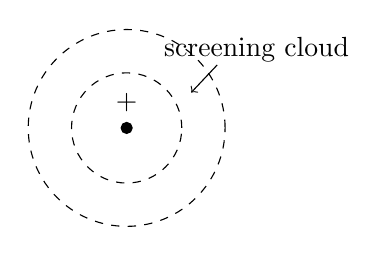
\begin{tikzpicture}[scale=1.0]
\draw[fill=black] (0,0) circle (0.07);
\node[above] at (0,0.08) {\(+\)};
\draw[dashed] (0,0) circle (0.7);
\draw[dashed] (0,0) circle (1.25);
\node at (1.65,1.0) {screening cloud};
\draw[->] (1.15,0.8) -- (0.82,0.45);
\end{tikzpicture}
\caption{Schematic screening picture: at shorter distance more of the cloud is peeled away, so the effective QED charge increases.}
\end{figure}

The specifically quantum statement is then this. The vacuum contains virtual pairs at all energies, hence at all effective sizes. As we probe at smaller and smaller \(r\), we peel away more and more of the screening cloud. The effective charge therefore depends on scale:
\begin{equation}
e=e(r)\qquad\text{or equivalently}\qquad e=e(1/r).
\end{equation}
And the lecture stresses that in QED this increase is slow, logarithmic, but persistent. The more finely we probe, the larger the charge appears.

\paragraph{QCD antiscreening.}
The strong interaction does the opposite. Because gluons interact with gluons, the chromoelectric flux lines attract one another and are squeezed into tube-like structures. At large separation the potential is therefore approximately linear:
\begin{equation}
V_{\mathrm{QCD}}(r)\propto r.
\end{equation}
That is confinement in the language of the lecture.

\begin{figure}[h]
\centering
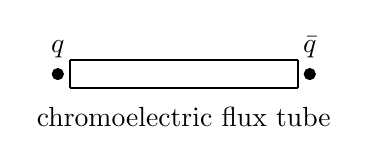
\begin{tikzpicture}[scale=1.0]
\draw[fill=black] (-1.6,0) circle (0.07);
\draw[fill=black] (1.6,0) circle (0.07);
\node[above] at (-1.6,0.08) {\(q\)};
\node[above] at (1.6,0.08) {\(\bar q\)};
\draw[thick] (-1.45,0.18) -- (1.45,0.18);
\draw[thick] (-1.45,-0.18) -- (1.45,-0.18);
\draw[thick] (-1.45,0.18) -- (-1.45,-0.18);
\draw[thick] (1.45,0.18) -- (1.45,-0.18);
\node at (0,-0.55) {chromoelectric flux tube};
\end{tikzpicture}
\caption{A schematic QCD flux tube: at large separation the energy grows linearly with \(r\).}
\end{figure}

In this language the effective strong coupling grows with separation and decreases with inverse separation. So if QED slowly rises as we go to shorter distance, QCD falls.

\paragraph{Weak coupling and the unification scale.}
The weak coupling lies in between. Susskind's point is qualitative but central: if we take the measured couplings at accessible energies and run them upward using the Standard Model, the electromagnetic, weak, and strong couplings come close to meeting. In supersymmetric extensions they meet more sharply, at an energy of order
\begin{equation}
\mu_{\mathrm{unif}}\sim 10^{16}\,\mathrm{GeV}.
\end{equation}
The lecture is careful not to oversell this. It is not yet a theorem. It is an observation about numbers and the slow logarithmic running of the couplings. But it is exactly the sort of observation that makes one suspect a deeper unified structure at very high energy.

\begin{figure}[h]
\centering
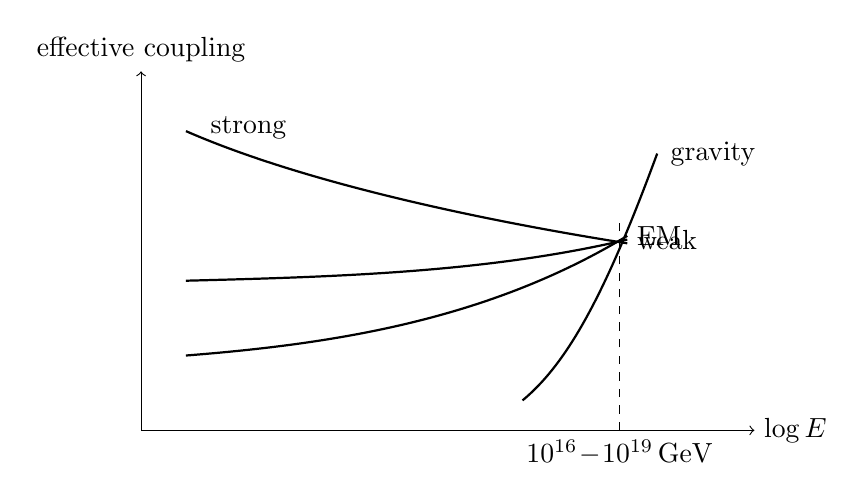
\begin{tikzpicture}[scale=0.95]
\draw[->] (0,0) -- (8.2,0) node[right] {\(\log E\)};
\draw[->] (0,0) -- (0,4.8) node[above] {effective coupling};

\draw[thick] (0.6,1.0) .. controls (2.5,1.15) and (4.6,1.45) .. (6.5,2.6);
\node[right] at (6.5,2.6) {EM};

\draw[thick] (0.6,2.0) .. controls (2.5,2.05) and (4.6,2.1) .. (6.5,2.55);
\node[right] at (6.5,2.55) {weak};

\draw[thick] (0.6,4.0) .. controls (2.2,3.3) and (4.6,2.8) .. (6.5,2.5);
\node[right] at (0.8,4.05) {strong};

\draw[thick] (5.1,0.4) .. controls (5.7,0.9) and (6.2,1.8) .. (6.9,3.7);
\node[right] at (6.95,3.7) {gravity};

\draw[dashed] (6.4,0) -- (6.4,2.8);
\node[below] at (6.4,0) {\(10^{16}\!-\!10^{19}\,\mathrm{GeV}\)};
\end{tikzpicture}
\caption{Qualitative running of the gauge couplings, together with the heuristic rise of gravity at short distance.}
\end{figure}

\paragraph{Short-distance gravity.}
The lecture then adds gravity heuristically. Here it is worth keeping the corrected distinction that Susskind himself makes on the board. If we use energy rather than rest mass in Newton's law, then for relativistic particles
\begin{equation}
F_G(r)\sim \frac{GE^2}{c^4r^2}.
\end{equation}
Now localizing a particle within distance \(r\) forces its momentum to be of order
\begin{equation}
p\sim \frac{\hbar}{r},
\qquad
E\sim pc\sim \frac{\hbar c}{r}.
\end{equation}
If we first think in terms of potential energy, then
\begin{equation}
U_G(r)\sim \frac{GE^2}{c^4r}
\sim
\frac{G\hbar^2}{c^2r^3}.
\end{equation}
This is the place where the lecture's spoken ``one over \(r^3\)'' belongs. But for the force itself one differentiates once more and finds
\begin{equation}
F_G(r)\sim \frac{G\hbar^2}{c^2r^4}.
\end{equation}
So at very short distances gravity grows faster than the Coulomb force. Comparing this with \(F_{\mathrm{Coulomb}}(r)\sim e^2/r^2\), one obtains the characteristic crossover scale
\begin{equation}
r_P\sim \sqrt{\frac{G\hbar}{c^3}},
\end{equation}
up to the lecture's rough simplification of the dimensionless electromagnetic coupling. That is the Planck length.

Now the lecture closes the circle. Once one admits very high scales such as the unification scale or the Planck scale, those high scales begin to look natural. The small scale is what becomes puzzling. Why is the electroweak scale, encoded in \(F\), so tiny by comparison? Why is the one number that controls the masses of the \(W\), the \(Z\), the quarks, and the charged leptons the exceptional small quantity in the theory?

That is the lecture's final serious theme. It is not solved. It is sharpened. And the sharpening matters: once we understand where the masses come from, the unresolved question is no longer how to write them down. It is why the scale that writes them down is so small.

\section{Summary}

The lecture proceeds by tightening one mathematical point after another. We begin with the Dirac Lagrangian, first in the older \(\alpha,\beta\) notation and then in the cleaner covariant language, in order to isolate what a Dirac mass term really does: it mixes left- and right-chiral fermions. Once the weak interaction is recalled to be chiral, that mass term becomes forbidden as a bare term in the Lagrangian. The Higgs field repairs the problem by carrying the needed weak charge, and after the shift \(\phi=F+H\) the Yukawa coupling splits into a fermion mass term and a Higgs interaction term. The Higgs potential then determines the scale \(F\) through \(F^2=\mu^2/\lambda\). That local success immediately opens the deeper question of the lecture: why is \(F\) so small compared with the natural ultraviolet scales suggested by running couplings, unification, and the Planck scale? The lecture ends, as it should, not by pretending that the hierarchy problem has been solved, but by making clear exactly where and why it arises.